\begin{enumerate}[label=\thesubsection.\arabic*.,ref=\thesubsection.\theenumi]
    \numberwithin{equation}{enumi}
    \numberwithin{figure}{enumi}

    \item A series-shunt feedback amplifier employs a basic amplifier with input and output resistances each of $2K\Omega$ and
    gain G = 1000V/V. The feedback factor H = 0.1V/V. Find the input resistance $R_{if}$, output resistance $R_{of}$ and gain 
    of the closed-loop amplifier. \\
    
\solution 
For given data, see Table:\ref{table:ee18btech11039_tab1}.
For feedback-amplifier circuit and equivalent circuit, see fig:\ref{fig:ee18btech11039_fig1} and \ref{fig:ee18btech11039_fig2}

\begin{table}[!h]
\centering
%%  This section checks if we are begin input into another file or  %%
%%  the file will be compiled alone. First use a macro taken from   %%
%%  the TeXbook ex 7.7 (suggestion of Han-Wen Nienhuys).            %%
\def\ifundefined#1{\expandafter\ifx\csname#1\endcsname\relax}


%%  Check for the \def token for inputed files. If it is not        %%
%%  defined, the file will be processed as a standalone and the     %%
%%  preamble will be used.                                          %%
\ifundefined{inputGnumericTable}

%%  We must be able to close or not the document at the end.        %%
	\def\gnumericTableEnd{\end{document}}


%%%%%%%%%%%%%%%%%%%%%%%%%%%%%%%%%%%%%%%%%%%%%%%%%%%%%%%%%%%%%%%%%%%%%%
%%                                                                  %%
%%  This is the PREAMBLE. Change these values to get the right      %%
%%  paper size and other niceties.                                  %%
%%                                                                  %%
%%%%%%%%%%%%%%%%%%%%%%%%%%%%%%%%%%%%%%%%%%%%%%%%%%%%%%%%%%%%%%%%%%%%%%

	\documentclass[12pt%
			  %,landscape%
                    ]{report}
       \usepackage[latin1]{inputenc}
       \usepackage{fullpage}
       \usepackage{color}
       \usepackage{array}
       \usepackage{longtable}
       \usepackage{calc}
       \usepackage{multirow}
       \usepackage{hhline}
       \usepackage{ifthen}
%%  End of the preamble for the standalone. The next section is for %%
%%  documents which are included into other LaTeX2e files.          %%
\else

%%  We are not a stand alone document. For a regular table, we will %%
%%  have no preamble and only define the closing to mean nothing.   %%
    \def\gnumericTableEnd{}

%%  If we want landscape mode in an embedded document, comment out  %%
%%  the line above and uncomment the two below. The table will      %%
%%  begin on a new page and run in landscape mode.                  %%
%       \def\gnumericTableEnd{\end{landscape}}
%       \begin{landscape}


%%  End of the else clause for this file being \input.              %%
\fi

%%%%%%%%%%%%%%%%%%%%%%%%%%%%%%%%%%%%%%%%%%%%%%%%%%%%%%%%%%%%%%%%%%%%%%
%%                                                                  %%
%%  The rest is the gnumeric table, except for the closing          %%
%%  statement. Changes below will alter the table's appearance.     %%
%%                                                                  %%
%%%%%%%%%%%%%%%%%%%%%%%%%%%%%%%%%%%%%%%%%%%%%%%%%%%%%%%%%%%%%%%%%%%%%%

\providecommand{\gnumericmathit}[1]{#1} 
%%  Uncomment the next line if you would like your numbers to be in %%
%%  italics if they are italizised in the gnumeric table.           %%
%\renewcommand{\gnumericmathit}[1]{\mathit{#1}}
\providecommand{\gnumericPB}[1]%
{\let\gnumericTemp=\\#1\let\\=\gnumericTemp\hspace{0pt}}
 \ifundefined{gnumericTableWidthDefined}
        \newlength{\gnumericTableWidth}
        \newlength{\gnumericTableWidthComplete}
        \newlength{\gnumericMultiRowLength}
        \global\def\gnumericTableWidthDefined{}
 \fi
%% The following setting protects this code from babel shorthands.  %%
 \ifthenelse{\isundefined{\languageshorthands}}{}{\languageshorthands{english}}
%%  The default table format retains the relative column widths of  %%
%%  gnumeric. They can easily be changed to c, r or l. In that case %%
%%  you may want to comment out the next line and uncomment the one %%
%%  thereafter                                                      %%
\providecommand\gnumbox{\makebox[0pt]}
%%\providecommand\gnumbox[1][]{\makebox}

%% to adjust positions in multirow situations                       %%
\setlength{\bigstrutjot}{\jot}
\setlength{\extrarowheight}{\doublerulesep}

%%  The \setlongtables command keeps column widths the same across  %%
%%  pages. Simply comment out next line for varying column widths.  %%
\setlongtables

\setlength\gnumericTableWidth{%
	50pt+%
	50pt+%
	50pt+%
0pt}
\def\gumericNumCols{3}
\setlength\gnumericTableWidthComplete{\gnumericTableWidth+%
         \tabcolsep*\gumericNumCols*2+\arrayrulewidth*\gumericNumCols}
\ifthenelse{\lengthtest{\gnumericTableWidthComplete > \linewidth}}%
         {\def\gnumericScale{\ratio{\linewidth-%
                        \tabcolsep*\gumericNumCols*2-%
                        \arrayrulewidth*\gumericNumCols}%
{\gnumericTableWidth}}}%
{\def\gnumericScale{1}}

%%%%%%%%%%%%%%%%%%%%%%%%%%%%%%%%%%%%%%%%%%%%%%%%%%%%%%%%%%%%%%%%%%%%%%
%%                                                                  %%
%% The following are the widths of the various columns. We are      %%
%% defining them here because then they are easier to change.       %%
%% Depending on the cell formats we may use them more than once.    %%
%%                                                                  %%
%%%%%%%%%%%%%%%%%%%%%%%%%%%%%%%%%%%%%%%%%%%%%%%%%%%%%%%%%%%%%%%%%%%%%%

\ifthenelse{\isundefined{\gnumericColA}}{\newlength{\gnumericColA}}{}\settowidth{\gnumericColA}{\begin{tabular}{@{}p{50pt*\gnumericScale}@{}}x\end{tabular}}
\ifthenelse{\isundefined{\gnumericColB}}{\newlength{\gnumericColB}}{}\settowidth{\gnumericColB}{\begin{tabular}{@{}p{60pt*\gnumericScale}@{}}x\end{tabular}}
\ifthenelse{\isundefined{\gnumericColC}}{\newlength{\gnumericColC}}{}\settowidth{\gnumericColC}{\begin{tabular}{@{}p{60pt*\gnumericScale}@{}}x\end{tabular}}

\begin{tabular}[c]{%
	b{\gnumericColA}%
	b{\gnumericColB}%
	b{\gnumericColC}%
	}

%%%%%%%%%%%%%%%%%%%%%%%%%%%%%%%%%%%%%%%%%%%%%%%%%%%%%%%%%%%%%%%%%%%%%%
%%  The longtable options. (Caption, headers... see Goosens, p.124) %%
%	\caption{The Table Caption.}             \\	%
% \hline	% Across the top of the table.
%%  The rest of these options are table rows which are placed on    %%
%%  the first, last or every page. Use \multicolumn if you want.    %%

%%  Header for the first page.                                      %%
%	\multicolumn{3}{c}{The First Header} \\ \hline 
%	\multicolumn{1}{c}{colTag}	%Column 1
%	&\multicolumn{1}{c}{colTag}	%Column 2
%	&\multicolumn{1}{c}{colTag}	\\ \hline %Last column
%	\endfirsthead

%%  The running header definition.                                  %%
%	\hline
%	\multicolumn{3}{l}{\ldots\small\slshape continued} \\ \hline
%	\multicolumn{1}{c}{colTag}	%Column 1
%	&\multicolumn{1}{c}{colTag}	%Column 2
%	&\multicolumn{1}{c}{colTag}	\\ \hline %Last column
%	\endhead

%%  The running footer definition.                                  %%
%	\hline
%	\multicolumn{3}{r}{\small\slshape continued\ldots} \\
%	\endfoot

%%  The ending footer definition.                                   %%
%	\multicolumn{3}{c}{That's all folks} \\ \hline 
%	\endlastfoot
%%%%%%%%%%%%%%%%%%%%%%%%%%%%%%%%%%%%%%%%%%%%%%%%%%%%%%%%%%%%%%%%%%%%%%

\hhline{|-|-|-}
	 \multicolumn{1}{|p{\gnumericColA}|}%
	{\gnumericPB{\centering}\textbf{Parameters}}
	&\multicolumn{1}{p{\gnumericColB}|}%
	{\gnumericPB{\centering}\textbf{Definition}}
	&\multicolumn{1}{p{\gnumericColC}|}%
	{\gnumericPB{\centering}\textbf{For given circuit}}

	
\\


\hhline{|---|}
	 \multicolumn{1}{|p{\gnumericColA}|}%
	{\gnumericPB{\centering}{Open loop gain}}
	&\multicolumn{1}{p{\gnumericColB}|}%
	{\gnumericPB{\centering}G}
	&\multicolumn{1}{p{\gnumericColC}|}%
	{\gnumericPB{\centering}1000}

\\
\hhline{|---|}
	 \multicolumn{1}{|p{\gnumericColA}|}%
	{\gnumericPB{\centering}Feedback factor}
	&\multicolumn{1}{p{\gnumericColB}|}%
	{\gnumericPB{\centering}H}
	&\multicolumn{1}{p{\gnumericColC}|}%
	{\gnumericPB{\centering}0.1}

\\
\hhline{|---|}
	 \multicolumn{1}{|p{\gnumericColA}|}%
	{\gnumericPB{\centering}Open-loop input resistance}
	&\multicolumn{1}{p{\gnumericColB}|}%
	{\gnumericPB{\centering}$R_i$}
	&\multicolumn{1}{p{\gnumericColC}|}%
	{\gnumericPB{\centering}$2K\Omega$}

\\
\hhline{|---|}
	 \multicolumn{1}{|p{\gnumericColA}|}%
	{\gnumericPB{\centering}Open-loop output resistance}
	&\multicolumn{1}{p{\gnumericColB}|}%
	{\gnumericPB{\centering}$R_o$}
	&\multicolumn{1}{p{\gnumericColC}|}%
	{\gnumericPB{\centering}$2K\Omega$}

\\
\hhline{|---|}
\end{tabular}

\ifthenelse{\isundefined{\languageshorthands}}{}{\languageshorthands{\languagename}}
\gnumericTableEnd
\caption{}
\label{table:ee18btech11039_tab1}
\end{table}

\begin{figure}[!h]
		\resizebox{\columnwidth}{!}{\begin{circuitikz}[american]
    
    \ctikzset{tripoles/mos style/arrows}
    \draw(0,0) to [resistor,l = $R_s$] (2,0) --(3,0)--(3,-1) to [resistor,l = $R_{id}$,v>=$V_1$](3,-3);
    \draw (3,-3) to [resistor,l = $R_1//R_2$] (0,-3);
    \draw(0,0) to [open,v>=$V_f$](0,-3);
    \draw(3,0) to [open] (4,0);
    \draw (4,0)--(5,0) to [resistor,l = $ r_o$] (6,0)--(6.5,0);
    \draw(6.5,0) to [resistor,l = $R_1+R_2$](6.5,-3);
    \draw(6.5,-3) node [ground]{};
    \draw(6.5,0)--(8.5,0)to [resistor,l = $R_L$] (8.5,-3);
    \draw(8.5,-3)node [ground]{};
    \draw(4,0)to [cV,l = $\mu V_1$] (4,-3);
    \draw(4,-3) node[ground]{};
    \draw(8.5,0)node[circle,fill,inner sep = 2pt,label = $V_o$]{};
    \end{circuitikz}
 }
\caption{Ideal structure}
\label{fig:ee18btech11039_fig1}
\end{figure}

\begin{figure}[!h]
		\resizebox{\columnwidth}{!}{\begin{circuitikz}[american]
    \ctikzset{tripoles/mos style/arrows}
    \draw (0, 0)--(2, 0) to[resistor, l = $R_{if}$] (2, -3)--(0, -3)
    \draw (0, 0) to[V, l = $V_i$, *-*] (0, -3);
    \draw (8, 0) to[short] (6, 0) to[resistor, l = $R_{of}$] (4, 0) to[cV, l = $TV_i$] (4, -3)--(8, -3) to[open, v^<=$V_o$, *-*](8, 0);
    \draw[dashed] (1.5, 0.5)--(6, 0.5)--(6, -3.5)--(1.5, -3.5)--(1.5, 0.5)
    (3.5, 0.5) node[above]{T-circuit};
    \end{circuitikz}}
\caption{Equivalent circuit}
\label{fig:ee18btech11039_fig2}
\end{figure}

Closed-loop gain,
\begin{align}
    T = \frac{G}{1+GH}
      = 9.9
\end{align}

\text{Input resistance,}
\begin{align}
    R_{if} = \brak{1+GH} R_i
    = 202K\Omega
\end{align}

\text{Output resistance,} 
\begin{align}
    R_{of} = \frac{R_o}{1+GH}
           = 19.802\Omega
\end{align}

\begin{figure}[!h]
		\resizebox{\columnwidth}{!}{\begin{circuitikz}[american]
    \ctikzset{tripoles/mos style/arrows}
    \draw (0, 0) to[V, l = $V_s$] (0, -2)node[ground]{}; 
    \draw (0, 0) to[resistor, l = $R_s$] (2, 0)--(4, 0)to[resistor, l = $R_{id}$, v>=$V_1$](4, -2.5)--(2, -2.5)--(2, -7)--(2.5, -7) to[resistor, l = $R_1$, *-] (2.5, -9) node[ground]{};
    \draw (2.5, -7) to[resistor, l = $R_2$](10, -7)--(10, -1)--(11, -1)to[resistor, l = $R_L$](11, -3)node[ground]{};
    \draw (11, -1)to[short, -*](12, -1)node[label = $V_o$]{};
    \draw (10, -1) to[resistor, l_= $r_o$] (7, -1) to[cV, l = $\mu V_1$] (7, -2.2)node[ground]{};
    \draw (3, 2.5)--(3, -5)--(9.8, -1)--(3, 2.5);
    \draw (6, 0)node[above]{op-amp};
    %--to[resistor, l = $R_1$]--(3.5, -3)node[ground]{};
    \end{circuitikz}}
\caption{Amplifier design}
\label{fig:ee18btech11039_fig3}
\end{figure}

\begin{figure}[!h]
		\resizebox{\columnwidth}{!}{\begin{circuitikz}[american]
    \ctikzset{tripoles/mos style/arrows}
    \draw (0, 0)to[resistor, l = $R_s$] (4, 0)to[resistor, l = $R_{id}$, v>=$V_1$] (4, -2)to[resistor, l = \mbox{$R_{11} = (R_1||R_2)$}](0, -2);
    %\draw (1.7, -2.1)node[anchor = north]{$R_{11} = (R_1||R_2)$};
    \draw (0, 0)to[open, v>= $V_i$, *-*] (0, -2);
    \draw (14, 0)node[circle,fill,inner sep=2pt, label = right:$V_o$]{}--(12, 0)to[resistor, l = \mbox{$R_{22} = (R_1+R_2)$}](12, -2)node[ground]{};
    \draw (12, 0)--(10, 0)to[resistor, l = $R_L$](10, -2)node[ground]{};
    \draw (10, 0)to[resistor, l = $r_o$](7, 0)to[cV, l = $\mu V_1$](7, -2)node[ground]{};
    ;
    \end{circuitikz}}
\caption{G circuit}
\label{fig:ee18btech11039_fig4}
\end{figure}

\begin{figure}[!h]
		\resizebox{\columnwidth}{!}{\begin{circuitikz}[american]
    \ctikzset{tripoles/mos style/arrows}
    \draw (0, -2)to[open, v^<=$V_f$, *-*](0, 0)to[short, i = \mbox{$I = 0$}](2, 0)--(2.5, 0)to[resistor, l = $R_2$](5, 0)to[open, v^>=$V_o$, *-*](5, -2)--(2.5, -2)node[ground]{};
    \draw (2.5, 0)to[resistor, l = $R_1$, *-*](2.5, -2)--(0, -2);
    \end{circuitikz}}
\caption{H circuit}
\label{fig:ee18btech11039_fig5}
\end{figure}

\begin{table}[!h]
\centering
%%  This section checks if we are begin input into another file or  %%
%%  the file will be compiled alone. First use a macro taken from   %%
%%  the TeXbook ex 7.7 (suggestion of Han-Wen Nienhuys).            %%
\def\ifundefined#1{\expandafter\ifx\csname#1\endcsname\relax}


%%  Check for the \def token for inputed files. If it is not        %%
%%  defined, the file will be processed as a standalone and the     %%
%%  preamble will be used.                                          %%
\ifundefined{inputGnumericTable}

%%  We must be able to close or not the document at the end.        %%
	\def\gnumericTableEnd{\end{document}}


%%%%%%%%%%%%%%%%%%%%%%%%%%%%%%%%%%%%%%%%%%%%%%%%%%%%%%%%%%%%%%%%%%%%%%
%%                                                                  %%
%%  This is the PREAMBLE. Change these values to get the right      %%
%%  paper size and other niceties.                                  %%
%%                                                                  %%
%%%%%%%%%%%%%%%%%%%%%%%%%%%%%%%%%%%%%%%%%%%%%%%%%%%%%%%%%%%%%%%%%%%%%%

	\documentclass[12pt%
			  %,landscape%
                    ]{report}
       \usepackage[latin1]{inputenc}
       \usepackage{fullpage}
       \usepackage{color}
       \usepackage{array}
       \usepackage{longtable}
       \usepackage{calc}
       \usepackage{multirow}
       \usepackage{hhline}
       \usepackage{ifthen}
%%  End of the preamble for the standalone. The next section is for %%
%%  documents which are included into other LaTeX2e files.          %%
\else

%%  We are not a stand alone document. For a regular table, we will %%
%%  have no preamble and only define the closing to mean nothing.   %%
    \def\gnumericTableEnd{}

%%  If we want landscape mode in an embedded document, comment out  %%
%%  the line above and uncomment the two below. The table will      %%
%%  begin on a new page and run in landscape mode.                  %%
%       \def\gnumericTableEnd{\end{landscape}}
%       \begin{landscape}


%%  End of the else clause for this file being \input.              %%
\fi

%%%%%%%%%%%%%%%%%%%%%%%%%%%%%%%%%%%%%%%%%%%%%%%%%%%%%%%%%%%%%%%%%%%%%%
%%                                                                  %%
%%  The rest is the gnumeric table, except for the closing          %%
%%  statement. Changes below will alter the table's appearance.     %%
%%                                                                  %%
%%%%%%%%%%%%%%%%%%%%%%%%%%%%%%%%%%%%%%%%%%%%%%%%%%%%%%%%%%%%%%%%%%%%%%

\providecommand{\gnumericmathit}[1]{#1} 
%%  Uncomment the next line if you would like your numbers to be in %%
%%  italics if they are italizised in the gnumeric table.           %%
%\renewcommand{\gnumericmathit}[1]{\mathit{#1}}
\providecommand{\gnumericPB}[1]%
{\let\gnumericTemp=\\#1\let\\=\gnumericTemp\hspace{0pt}}
 \ifundefined{gnumericTableWidthDefined}
        \newlength{\gnumericTableWidth}
        \newlength{\gnumericTableWidthComplete}
        \newlength{\gnumericMultiRowLength}
        \global\def\gnumericTableWidthDefined{}
 \fi
%% The following setting protects this code from babel shorthands.  %%
 \ifthenelse{\isundefined{\languageshorthands}}{}{\languageshorthands{english}}
%%  The default table format retains the relative column widths of  %%
%%  gnumeric. They can easily be changed to c, r or l. In that case %%
%%  you may want to comment out the next line and uncomment the one %%
%%  thereafter                                                      %%
\providecommand\gnumbox{\makebox[0pt]}
%%\providecommand\gnumbox[1][]{\makebox}

%% to adjust positions in multirow situations                       %%
\setlength{\bigstrutjot}{\jot}
\setlength{\extrarowheight}{\doublerulesep}

%%  The \setlongtables command keeps column widths the same across  %%
%%  pages. Simply comment out next line for varying column widths.  %%
\setlongtables

\setlength\gnumericTableWidth{%
	50pt+%
	50pt+%
	50pt+%
0pt}
\def\gumericNumCols{3}
\setlength\gnumericTableWidthComplete{\gnumericTableWidth+%
         \tabcolsep*\gumericNumCols*2+\arrayrulewidth*\gumericNumCols}
\ifthenelse{\lengthtest{\gnumericTableWidthComplete > \linewidth}}%
         {\def\gnumericScale{\ratio{\linewidth-%
                        \tabcolsep*\gumericNumCols*2-%
                        \arrayrulewidth*\gumericNumCols}%
{\gnumericTableWidth}}}%
{\def\gnumericScale{1}}

%%%%%%%%%%%%%%%%%%%%%%%%%%%%%%%%%%%%%%%%%%%%%%%%%%%%%%%%%%%%%%%%%%%%%%
%%                                                                  %%
%% The following are the widths of the various columns. We are      %%
%% defining them here because then they are easier to change.       %%
%% Depending on the cell formats we may use them more than once.    %%
%%                                                                  %%
%%%%%%%%%%%%%%%%%%%%%%%%%%%%%%%%%%%%%%%%%%%%%%%%%%%%%%%%%%%%%%%%%%%%%%

\ifthenelse{\isundefined{\gnumericColA}}{\newlength{\gnumericColA}}{}\settowidth{\gnumericColA}{\begin{tabular}{@{}p{50pt*\gnumericScale}@{}}x\end{tabular}}
\ifthenelse{\isundefined{\gnumericColB}}{\newlength{\gnumericColB}}{}\settowidth{\gnumericColB}{\begin{tabular}{@{}p{60pt*\gnumericScale}@{}}x\end{tabular}}
\ifthenelse{\isundefined{\gnumericColC}}{\newlength{\gnumericColC}}{}\settowidth{\gnumericColC}{\begin{tabular}{@{}p{60pt*\gnumericScale}@{}}x\end{tabular}}

\begin{tabular}[c]{%
	b{\gnumericColA}%
	b{\gnumericColB}%
	b{\gnumericColC}%
	}

%%%%%%%%%%%%%%%%%%%%%%%%%%%%%%%%%%%%%%%%%%%%%%%%%%%%%%%%%%%%%%%%%%%%%%
%%  The longtable options. (Caption, headers... see Goosens, p.124) %%
%	\caption{The Table Caption.}             \\	%
% \hline	% Across the top of the table.
%%  The rest of these options are table rows which are placed on    %%
%%  the first, last or every page. Use \multicolumn if you want.    %%

%%  Header for the first page.                                      %%
%	\multicolumn{3}{c}{The First Header} \\ \hline 
%	\multicolumn{1}{c}{colTag}	%Column 1
%	&\multicolumn{1}{c}{colTag}	%Column 2
%	&\multicolumn{1}{c}{colTag}	\\ \hline %Last column
%	\endfirsthead

%%  The running header definition.                                  %%
%	\hline
%	\multicolumn{3}{l}{\ldots\small\slshape continued} \\ \hline
%	\multicolumn{1}{c}{colTag}	%Column 1
%	&\multicolumn{1}{c}{colTag}	%Column 2
%	&\multicolumn{1}{c}{colTag}	\\ \hline %Last column
%	\endhead

%%  The running footer definition.                                  %%
%	\hline
%	\multicolumn{3}{r}{\small\slshape continued\ldots} \\
%	\endfoot

%%  The ending footer definition.                                   %%
%	\multicolumn{3}{c}{That's all folks} \\ \hline 
%	\endlastfoot
%%%%%%%%%%%%%%%%%%%%%%%%%%%%%%%%%%%%%%%%%%%%%%%%%%%%%%%%%%%%%%%%%%%%%%

\hhline{|-|-|-}
	 \multicolumn{1}{|p{\gnumericColA}|}%
	{\gnumericPB{\centering}\textbf{Parameter}}
	&\multicolumn{1}{p{\gnumericColC}|}%
	{\gnumericPB{\centering}\textbf{Value}}

	
\\


\hhline{|---|}
	 \multicolumn{1}{|p{\gnumericColA}|}%
	{\gnumericPB{\centering}{Op-amp gain$\brak{\mu}$}}
	&\multicolumn{1}{p{\gnumericColC}|}%
	{\gnumericPB{\centering}$10^4$}

\\
\hhline{|---|}
	 \multicolumn{1}{|p{\gnumericColA}|}%
	{\gnumericPB{\centering}{$R_s$}}
	&\multicolumn{1}{p{\gnumericColC}|}%
	{\gnumericPB{\centering}$100\ohm$}

\\
\hhline{|---|}
	 \multicolumn{1}{|p{\gnumericColA}|}%
	{\gnumericPB{\centering}{$R_{id}$}}
	&\multicolumn{1}{p{\gnumericColC}|}%
	{\gnumericPB{\centering}$1K\ohm$}

\\
\hhline{|---|}
	 \multicolumn{1}{|p{\gnumericColA}|}%
	{\gnumericPB{\centering}{$r_o$}}
	&\multicolumn{1}{p{\gnumericColC}|}%
	{\gnumericPB{\centering}$10K\ohm$}

\\
\hhline{|---|}
	 \multicolumn{1}{|p{\gnumericColA}|}%
	{\gnumericPB{\centering}{$R_1$}}
	&\multicolumn{1}{p{\gnumericColC}|}%
	{\gnumericPB{\centering}$1K\ohm$}
\\
\hhline{|---|}
	 \multicolumn{1}{|p{\gnumericColA}|}%
	{\gnumericPB{\centering}{$R_2$}}
	&\multicolumn{1}{p{\gnumericColC}|}%
	{\gnumericPB{\centering}$9K\ohm$}
\\
\hhline{|---|}
	 \multicolumn{1}{|p{\gnumericColA}|}%
	{\gnumericPB{\centering}{$R_L$}}
	&\multicolumn{1}{p{\gnumericColC}|}%
	{\gnumericPB{\centering}$3.33K\ohm$}
\\
\hhline{|---|}
\end{tabular}

\ifthenelse{\isundefined{\languageshorthands}}{}{\languageshorthands{\languagename}}
\gnumericTableEnd
\caption{Parameter values}
\label{table:ee18btech11039_tab2}
\end{table}

\textbf{Circuit design: }
From fig:\ref{fig:ee18btech11039_fig4}
\begin{align}
G = \mu \frac{R_L || \brak{R_1 + R_2}}{\sbrak{R_L || \brak{R_1 + R_2}}+r_o} \frac{R_{id}}{R_{id}+R_s+\brak{R_1||R_2}} = 1000
\end{align}

Open-loop input resistance,
\begin{align}
     R_i =  R_s + R_{id} + \brak{R_1 || R_2} = 2K\ohm
\end{align}

From fig:\ref{fig:ee18btech11039_fig5}
\begin{align}
H = \frac{V_f}{V_o} = \frac{R_1}{R_1 + R_2} = 0.1
\end{align}

Open-loop output resistance,
\begin{align}
      R_o = r_o || R_L || \brak{R_2 + R_1} = 2K\ohm
\end{align}

In fig.\ref{fig:ee18btech11039_fig6}, 
\begin{align}
    V_{s}\brak{t} = \sin\brak{2000\pi t} \\
    \Rightarrow V_{s}\brak{s} = \frac{2000\pi}{s^2 + \brak{2000\pi}^2}
\end{align}
\begin{align}
    V_{o}\brak{t} = 9.9\sin\brak{2000\pi t}\\
    \Rightarrow V_{o}\brak{s} = \frac{9.9\brak{2000\pi}}{s^2 + \brak{2000\pi}^2}
\end{align}
\begin{align}
    T = \left|\frac{V_o\brak{s}}{V_{s}\brak{s}}\right| = 9.9
\end{align}

\begin{figure}[!h]
		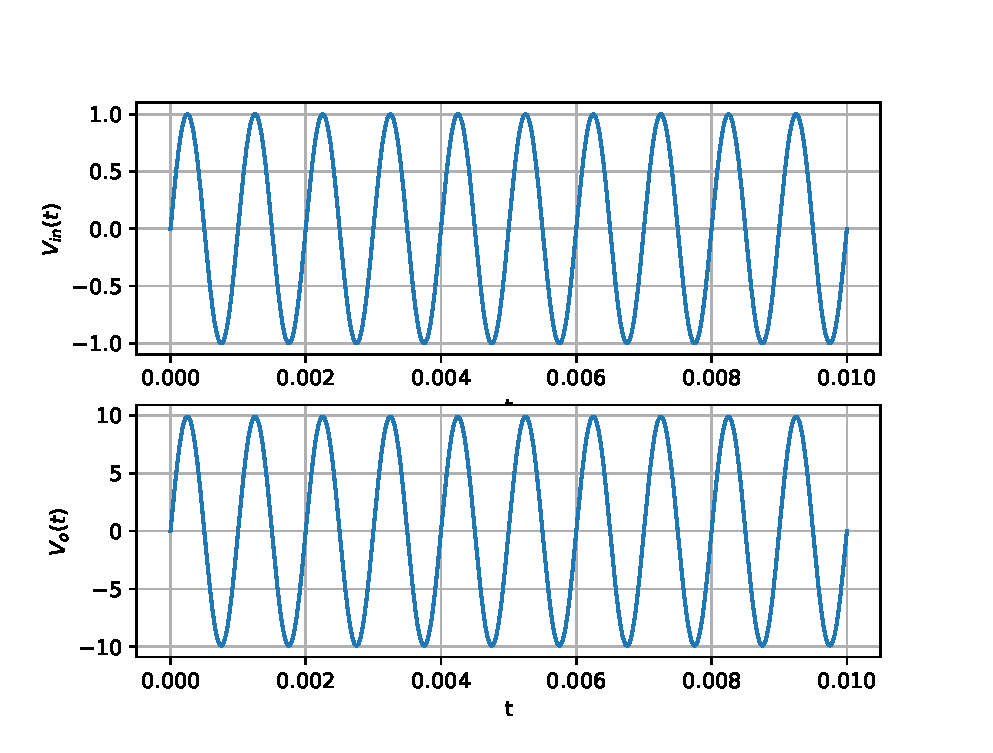
\includegraphics[width=\columnwidth]{./figs/ee18btech11039/spice_1.eps}
\caption{Time domain output of the simulation}
\label{fig:ee18btech11039_fig6}
\end{figure}

The plot in fig:\ref{fig:ee18btech11039_fig7} verifies that the value of T for the circuit is constant for various values of frequencies, $f \in \brak{1, 10^8}$.\\

The output in fig:\ref{fig:ee18btech11039_fig6} is obtained by running the following program-
\begin{lstlisting}
/codes/ee18btech11039/ee18btech11039_spice1.py
\end{lstlisting}
\begin{figure}[!h]
		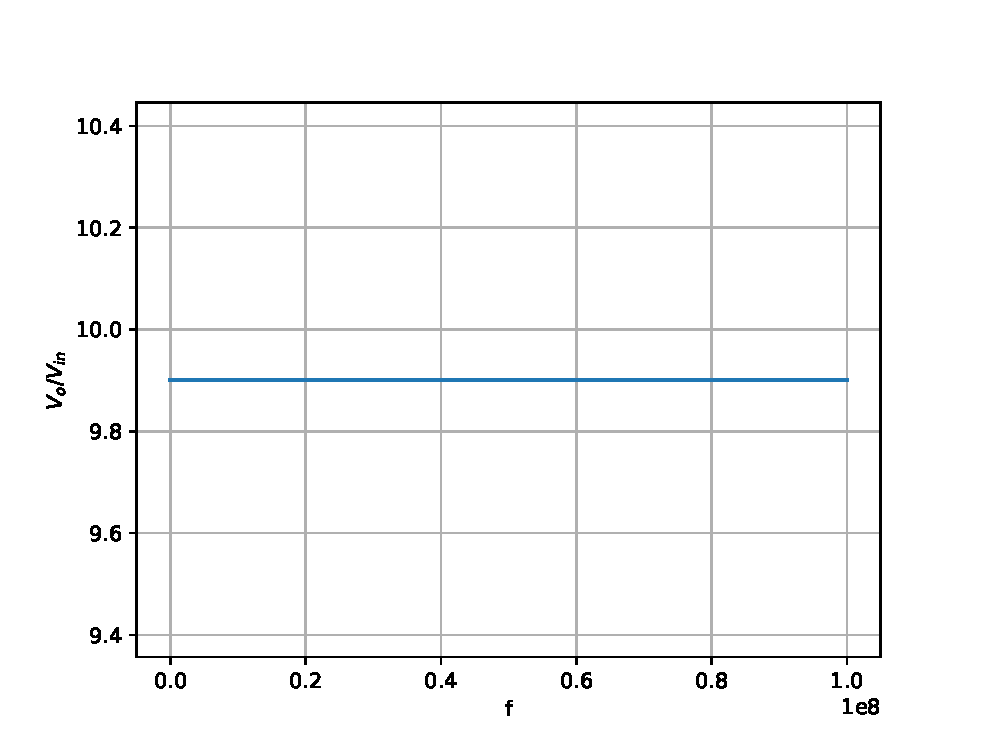
\includegraphics[width=\columnwidth]{./figs/ee18btech11039/spice_2.eps}
\caption{AC analysis, f = 1Hz to 100MHz}
\label{fig:ee18btech11039_fig7}
\end{figure}
 
The output in fig:\ref{fig:ee18btech11039_fig7} is obtained by running the following program-
\begin{lstlisting}
/codes/ee18btech11039/ee18btech11039_spice2.py
\end{lstlisting}
\end{enumerate}